\documentclass{article}
    % General document formatting
    \usepackage[margin=0.7in]{geometry}
    \usepackage[parfill]{parskip}
    \usepackage[utf8]{inputenc}
    \usepackage{amsmath}
    \usepackage{amssymb}
    \usepackage{tikz}
    \usepackage{fancyhdr}
    \usepackage{listings}

\pagestyle{fancy}
\fancyhf{}
\rhead{Edgar Jacob Rivera Rios - A01184125}

\begin{document}
\begin{titlepage}

    \newcommand{\HRule}{\rule{\linewidth}{0.5mm}} % Defines a new command for the horizontal lines, change thickness here

    \center % Center everything on the page

    %----------------------------------------------------------------------------------------
    %	HEADING SECTIONS
    %----------------------------------------------------------------------------------------

    \textsc{\LARGE Tecnológico de Monterrey}\\[1.5cm] % Name of your university/college
    \textsc{\Large Fundamentos de computación}\\[0.5cm] % Major heading such as course name
    %\textsc{\large Minor Heading}\\[0.5cm] % Minor heading such as course title

    %----------------------------------------------------------------------------------------
    %	TITLE SECTION
    %----------------------------------------------------------------------------------------

    \HRule \\[0.4cm]
    { \huge \bfseries Homework 5}\\[0.4cm] % Title of your document
    \HRule \\[1.5cm]

    %----------------------------------------------------------------------------------------
    %	AUTHOR SECTION
    %----------------------------------------------------------------------------------------

    \begin{minipage}{0.4\textwidth}
    \begin{flushleft} \large
    \emph{Student:}\\
    Jacob \textsc{Rivera} % Your name
    \end{flushleft}
    \end{minipage}
    ~
    \begin{minipage}{0.4\textwidth}
    \begin{flushright} \large
    \emph{Professor:} \\
    Dr. Hugo \textsc{Terashima} % Supervisor's Name
    \end{flushright}
    \end{minipage}\\[2cm]

    % If you don't want a supervisor, uncomment the two lines below and remove the section above
    %\Large \emph{Author:}\\
    %John \textsc{Smith}\\[3cm] % Your name

    %----------------------------------------------------------------------------------------
    %	DATE SECTION
    %----------------------------------------------------------------------------------------

    {\large \today}\\[2cm] % Date, change the \today to a set date if you want to be precise

    %----------------------------------------------------------------------------------------
    %	LOGO SECTION
    %----------------------------------------------------------------------------------------

    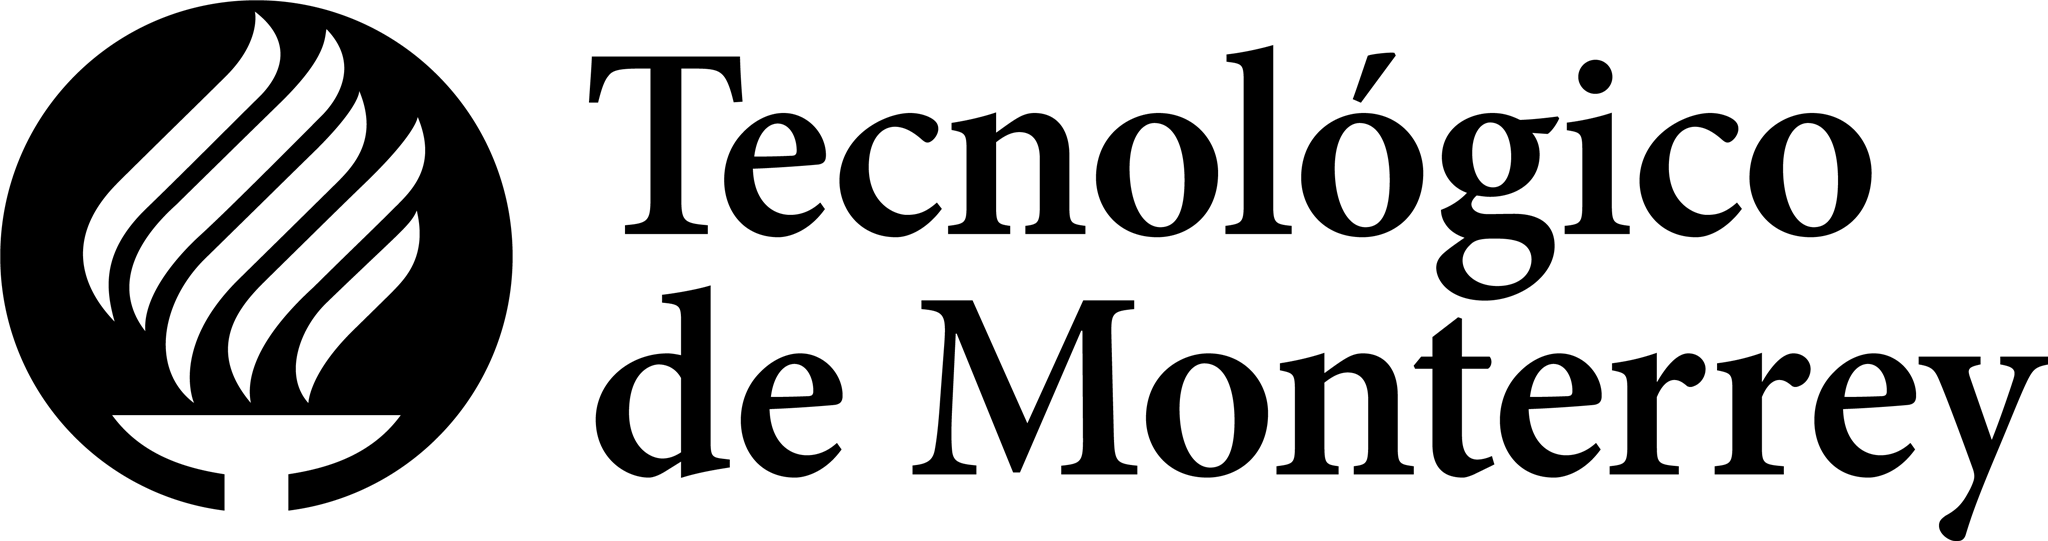
\includegraphics[width=0.4\textwidth,height=\textheight,keepaspectratio]{logo-tec-negro.png} % Include a department/university logo - this will require the graphicx package

    %----------------------------------------------------------------------------------------

    \vfill % Fill the rest of the page with whitespace

\end{titlepage}


\section{Problems}
Solve the following problems:
\begin{enumerate}
    \item Implement algorithms quicksort, mergesort and heapsort in any programming language, and investigate their performance in arrays of size $10^2$, $10^3$, $10^4$, $10^5$ and $10^6$. For each of those sizes, consider files of  randomly-generated  integers,  files  with  integers  already  sorted  in  ascending  order,  and  files  with integers already sorted in descending order. Hand in a report with your investigation containing the analysis, discussion of results and the conclusions.
    \begin{enumerate}
        \item Results\\
        The implementations where used in the Rust language, a low level language with data safety. As such implementation were pretty fast.
        The test was taken by repeating the sorting process 30 times for each combination and obtaining the mean.\\
        \begin{tabular}{|c|c|c|c|c|c|c|c|c|c|}
            \hline
            &Quick &Quick &Quick &Heap &Heap &Heap &Merge &Merge &Merge\\
            &Random &Ordered &Reverse &Random &Ordered &Reverse &Random &Ordered &Reverse\\
            \hline
            $10^2$& $1.75e^{-5}$s & $1.29e^{-5}$s & $1.38e^{-5}$s & $1.65e^{-6}$s & $1.70e^{-6}$s & $1.45e^{-6}$s & $2.49e^{-6}$s & $1.96e^{-6}$s & $1.95e^{-6}$s\\
            $10^3$& $1.98e^{-4}$s & $1.52e^{-4}$s & $1.58e^{-4}$s & $4.49e^{-5}$s & $3.68e^{-5}$s & $3.65e^{-5}$s & $5.43e^{-5}$s & $2.53e^{-5}$s & $2.46e^{-5}$s\\
            $10^4$& $2.22e^{-3}$s & $1.60e^{-3}$s & $1.67e^{-3}$s & $7.36e^{-4}$s & $4.78e^{-4}$s & $5.19e^{-4}$s & $8.57e^{-4}$s & $4.40e^{-4}$s & $3.24e^{-4}$s\\
            $10^5$& $2.42e^{-2}$s & $1.67e^{-2}$s & $1.75e^{-2}$s & $9.32e^{-3}$s & $5.63e^{-3}$s & $6.19e^{-3}$s & $1.15e^{-2}$s & $4.79e^{-3}$s & $3.75e^{-3}$s\\
            $10^6$& $0.257$s      & $0.178$s      & $0.184$s      & $0.119$s      & $6.16e^{-2}$s & $6.78e^{-2}$s & $0.132$s      & $5.74e^{-2}$s & $6.08e^{-2}$s\\
            \hline
        \end{tabular}

        \item Discussion\\
        We can see that the results in all 3 algorithms are pretty fast. However, by the nature of the language and the differences in implementation, we can see that in general merge and heap sort are faster than quick sort in general, heap sort being the fastest. The growth can be see clearly with the quicksort, which maintains a stable rate of growth at approximately $nlogn$ corresponding with the number of elements. As we grow the number of elements by an order of magnitude, the time taken to order them also grows by an order of magnitude plus a fraction of that. The same can be observed in the other algorithms, however, due to the implementation details, the jump seems greater, although it maintains a consistent rate.

        \item Conclusions\\
        With this results, we can see that the properties of each algorithm are maintained. The results are align with what we would look for each one. In general we see that the algorithms will perform similarly in the situations presented, which is analog on how the complexity of each one performs. So, choosing the adequate one depends in which type of data it's going to be used in.

        We can also see that in real life, implementation details are quite important to get the best result possible for an algorithm. The result of a deep copy of data or the use of a inadequate structure can have problematic effects in the performance of the algorithm. This is specially true for low level languages, as the memory allocation and cleaning is not that automatized, providing opportunity for better performance, but requiring a more explicit implementation.

    \end{enumerate}


    \item Consider the 3-ary heap, similar to the binary heap, except that a no-leaf node has 3 siblings
    \begin{enumerate}
        \item How would you represent a 3-ary heap in an array?\\
        The first item is the root, the next 3 are its' sons and the next 3 are its grandchildren
        \item What is the height of a 3-ary heap with $n$ elements, in terms of $d = 3$ and $n$?\\
        $log_{3}(n)$
        \item For an element in position $i$ in the heap, determine the position of its parent and siblings.\\
        $parent_i = array[(i-1)/3]$ while arrays start at 0 and $i \neq 0$\\
        $siblings_i = array[(parent_i * 3)+1)]$ to $array[((parent_i * 3)+3)]$
        \item In general terms, determine the complexity of a heap algorithm with these features.\\
        $O(3log_3 n)$

    \end{enumerate}

    \item Show how a set of $n$ positive integers between 1 and $n^2$ can be sorted in linear time\\
    In this case we can use a radix sort as the complexity for it is $O(wn)$, where $w$ is the length of the size of the type. As in this case we can assume that $w$ can be expressed as $log_n(n)$, which simplifies to 1, we can see that the complexity converts to $O(n)$
    \item Describe an algorithm that makes 42 comparisons for sorting 15 elements in the worst case (Donald Knuth, The Art of Computer Programming, Vol. 3). Show how the algorithm works using an example.
\end{enumerate}
\end{document}